%% LaTeX2e class for student theses
%% sections/content.tex
%% 
%% Karlsruhe Institute of Technology
%% Institute for Program Structures and Data Organization
%% Chair for Software Design and Quality (SDQ)
%%
%% Dr.-Ing. Erik Burger
%% burger@kit.edu
%%
%% Version 1.3, 2016-12-29

\chapter{Privacy Concept}
\label{ch:PrivacyConcept}

Many say: Data is the new oil and the most valuable resource there is. This shows how important the control of our personal data is. To achieve this, many players have to fulfill their obligations. On the one hand, the personal awareness of every user himself to only communicate the required and necessary information. On the other hand, the data handling institutes duty to guarantee legal compliance to laws like the EU’s general data protective regulations. While one can't act for the individual, we can provide tools and rules for institutions to help with legal compliance.

\section{General Concept}
\label{sec:PrivacyConcept:general}

The EU General Data Protective Regulations clearly states, that data of EU citizens have to be saved and processed within EU countries \cite{personaldata.2011}. Only a view countries with equal data protective laws are excepted from this constraint. As a consequence, one needs a simple data-flow analysis (\autoref{sec:RelatedWork:dataflow}) to know the data distribution in our software system. To put it straight, one needs to know, what kind of data are available on which server. This task got especially important, since distributed cloud systems are reality and data saved on "on premise" servers are becoming increasingly rare.

As mentioned in \autoref{sec:RelatedWork:dataflow}, the automated data-flow analysis on architecture level is still in its early stages and therefore not suited for practice. As a compromise we decided on manual data tagging. To ease the data tagging and analysis process, we decided to use the common well defined categories \cite{Schmieders.2015}:
%A growing and continuous research field is exploring and developing approaches for automated data-flow analysis. However, these are still very limited and are therefore not yet suited for practice (see \autoref{sec:RelatedWork:dataflow}). Due to these limitations, we need manual annotation of components.

\begin{itemize}
	\item \textbf{Type 0: Personal Information}: Data relates directly or indirectly to personal information. This is independent from encryption or pseudonymization. (e.g. call detail record)
	
	\item \textbf{Type 1: Personally Identifiable Information}:  Data does not contain personal information. However, by combining, fusing or analysing data sets, the personal data could be reconstructed for complete or partial personal information. (e.g. browser history without user)
	
	\item \textbf{Type 2: Anonymous Data}: Data does not contain any personal information. Even by extensive data analysis no direct or indirect personal information can be extracted. (e.g. shop inventory data)
	
	\label{sec:PrivacyConcept:dataprivacylevel}
\end{itemize}

These three categories are used, since many data do not contain any direct or indirect link onto private data, however still contain indicators onto private data. This means, they neither qualify for the type 0 category (Personal), nor for the type 2 category (Anonymous). For example an online shop wants to analyse which products usually get ordered together. The orders got anonymized by removing the customer and shipping address. Nevertheless, the time-stamp is required to get a timed evaluation factor. These data are not personal. However, combining and evaluating these with user-login-times, also non-personal data, privacy relevant data can be extracted. This also disqualifies them for Type 2, completely anonymous data \cite{Schmieders.}\cite{Schmieders.2015}.

Summarizing, a manual, categorized annotation approach to identify the system components privacy level is used. Based on this privacy level categorization, the analysis, whether a systems deployment is privacy compliant, can be performed.


\section{Deployment Constraints}
\label{sec:PrivacyConcept:deploymentrules}

How can one guarantee legal compliant distribution? As mentioned in \autoref{sec:Introduction:motivation}, personal data of EU citizens are only allowed to be processed, transferred or saved inside EU countries [...]. We argue that the following constraints, combined with correct manual annotation, are sufficient to accomplish this:

\begin{itemize}
	\label{enum:deployment_rules}
	\setlength\itemsep{0em}
	\item \textbf{Rule \#1}: Type 0 components must be deployed in a "save" geo-location.
	\item \textbf{Rule \#2}: Type 2 components can be deployed anywhere.
	\item \textbf{Rule \#3}: Type 1 components can be deployed anywhere.
	\item \textbf{Rule \#4}: Only deploy Type 1 components together in an "un-save" geo-location, if they receive their information (transitively) from the same Type 1 component.
	% Only deploy Type 1 components (x_1, x_2, ...) together in an "un-save" geo-location, if a connected set X containing at least (x_1, x_2, ...) with only type 1 or type 2 components exists, that has a maxium of one connection to a type 0 componont
\end{itemize}

\textit{Rule 1 \& 2} does not need any further explanation. \textit{Rule 3} states that Type 1 components can be deployed anywhere. This is due to the fact that Type 1 data should not contain any personal information. \textit{Rule 4} however limits this deployment. This constraint is necessary, because the combination of multiple Type 1 data streams could lead to privacy relevant information. If the data streams, however, have a common type 1 component as data source, the deployment can be considered privacy compliant.

The ideas is, when a depersonalised component (d) has a single edge to a personal component (p), and many edges to other depersonalised components (D), and the components (D) do not have any connection a personal categorized component, then they share the data passed via the connection between d and p, which can not be personal. Otherwise d would be categorized as personal. Note that data streams with type 2 components can be ignored, since - by definition - they don't get in contact with any privacy relevant data. 

We are aware, that these rules are over-approximations towards legal compliance. However, we are using a software architecture model as the only source of information. Therefore, detailed information about actual privacy symbiotic data streams are not available on this high level ob abstraction. Nevertheless, we argue, that these rules already help to identify illegal deployments and establish privacy compliant (re-)deployments.

\autoref{fig:example_depl:1}, \autoref{fig:example_depl:2} and \autoref{fig:example_depl:3} illustrate the different base scenarios applying to Rule 4. In the remainder of this section, we will elaborate their privacy compliance state by applying \autoref{enum:deployment_rules}, rule 4.

\begin{figure}[h]
	\centering
	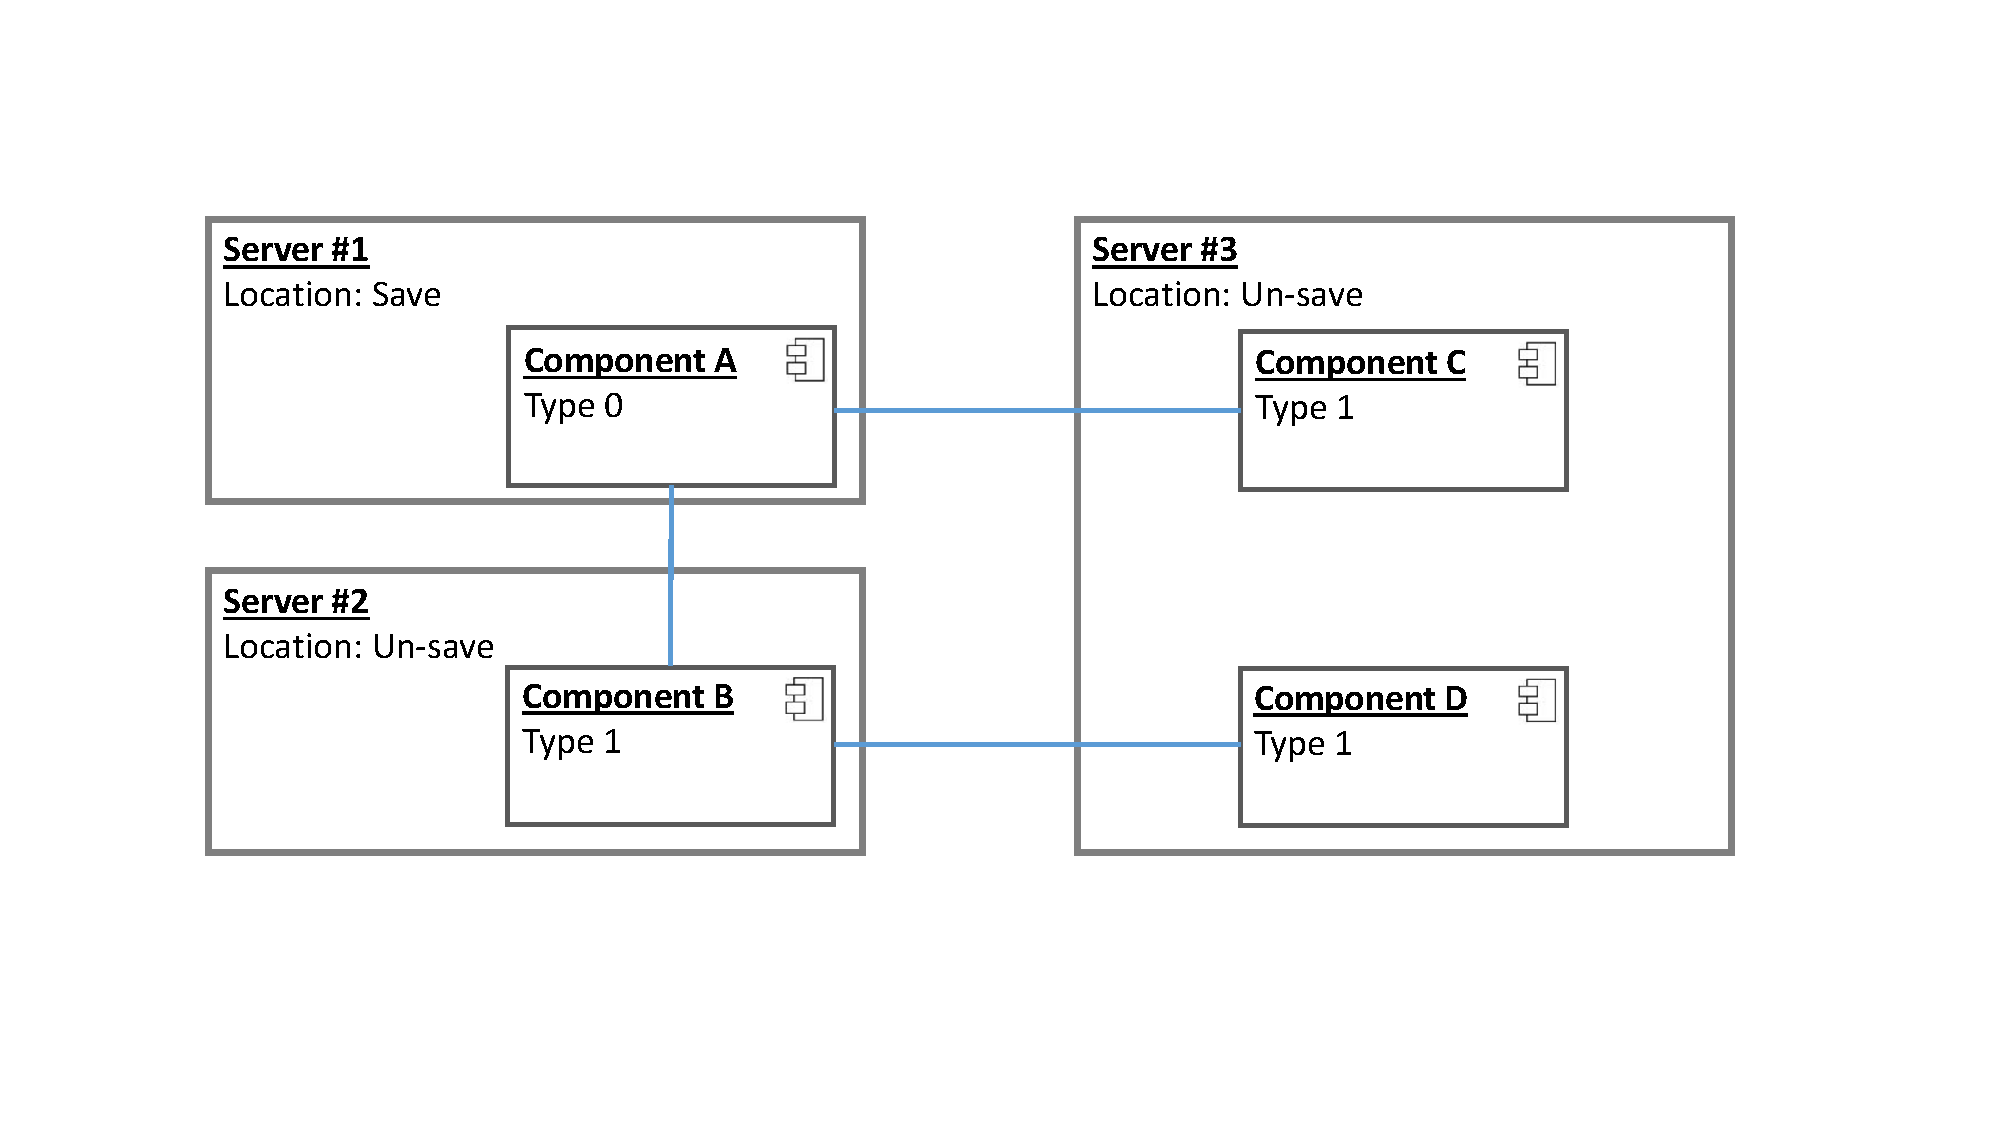
\includegraphics[trim = 35mm 45mm 40mm 30mm, clip, width=0.6\textwidth]{graphs/deployment_example_1}
	\caption{Privacy violating deployment}
	\label{fig:example_depl:1}
\end{figure}

The deployment shown in \autoref{fig:example_depl:1} is illegal. Server\#3 contains components with data streams from two different components, where one is a type 1 and one is a type 0 component. Even though A and C receives its data transitively from the same source, component A. This source is categorized as personal (type 0). Further, the data passes via different initial communication edges. As a result, \textit{Server \#3} hosts two type 1 components, which don't contain privacy relevant data by themselves. However, after combination, the data could be privacy relevant. So, this deployment is considered illegal.

\begin{figure}[h]
	\centering
	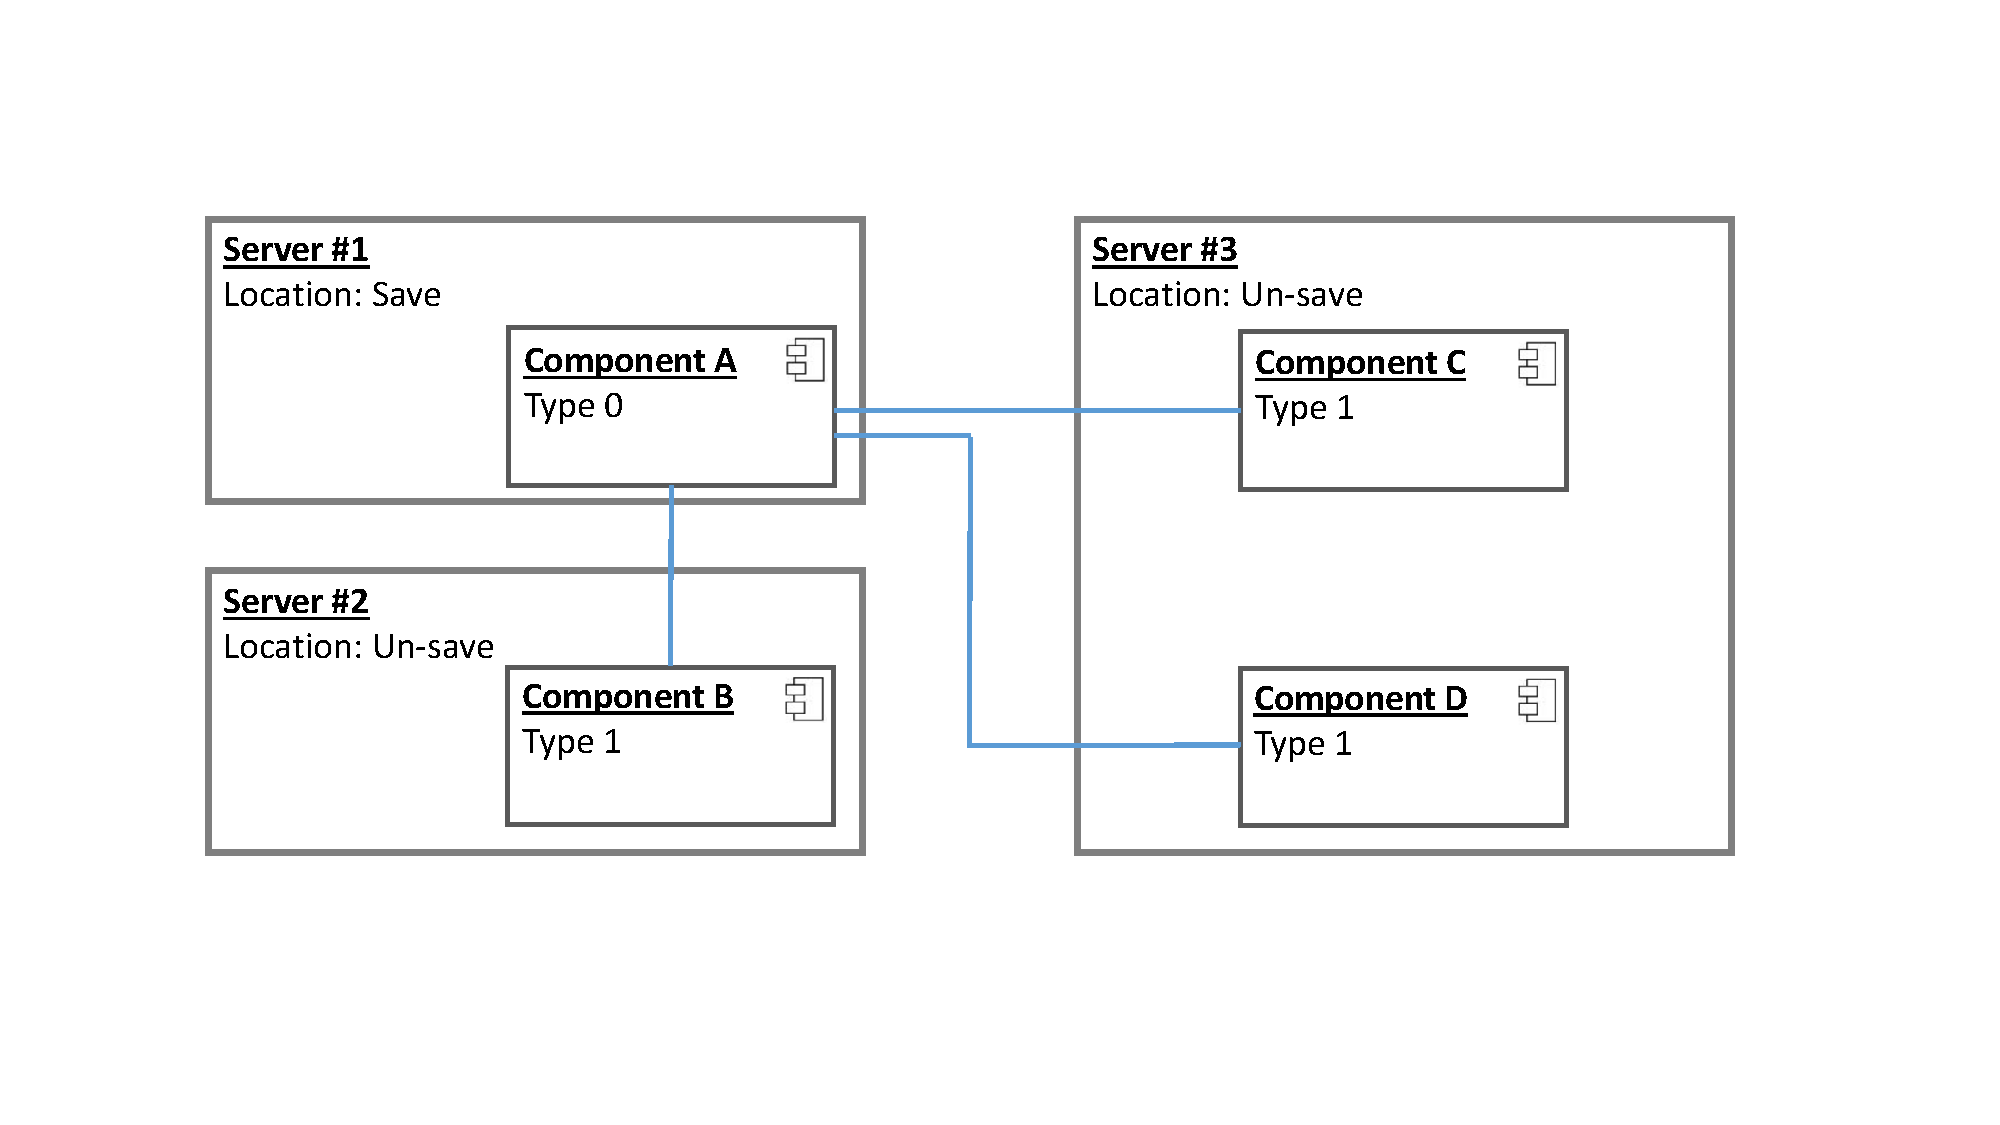
\includegraphics[trim = 35mm 45mm 40mm 30mm, clip, width=0.6\textwidth]{graphs/deployment_example_2}
	\caption{Privacy violating deployment}
	\label{fig:example_depl:2}
\end{figure}

\autoref{fig:example_depl:2} also shows an illegal considered deployment. Component C and D share the same data source, which is marked as type 0. As previously shown, the combination of data on Component C and D could lead to privacy relevant informations on \textit{Server \#3}.

\begin{figure}[h]
	\centering
	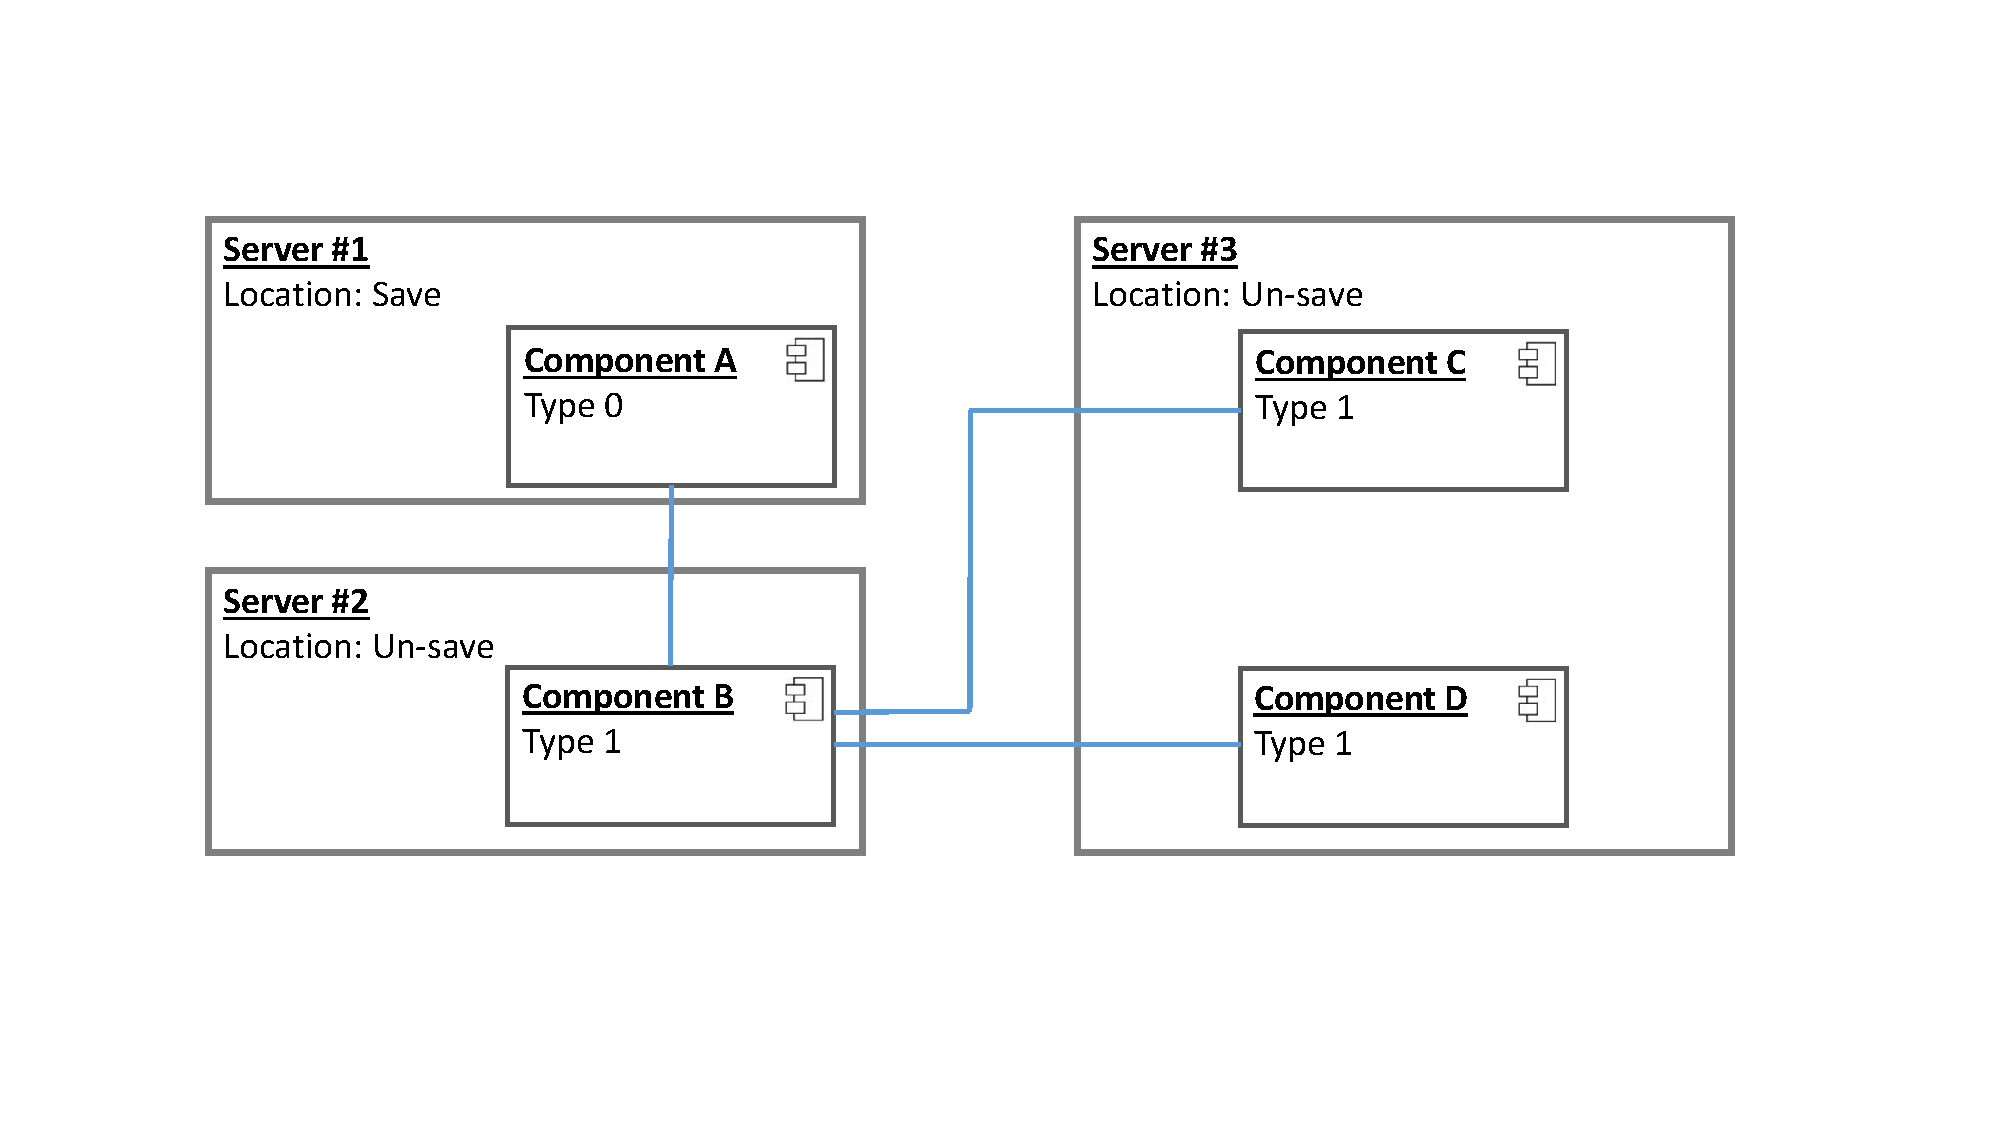
\includegraphics[trim = 35mm 45mm 40mm 35mm, clip, width=0.6\textwidth]{graphs/deployment_example_3}
	\caption{Privacy compliant deployment}
	\label{fig:example_depl:3}
\end{figure}

(\autoref{fig:example_depl:3}) shows a privacy compliant deployment. Due to, Component C and D sharing the same data source (Component B), which already only contains type 1 data. As a result, Component C and D can only contain data, already obtained by Component B. This means, even through data combination and extensive data analysis, no privacy concerning information can be extracted.


\section{Component categorization}
\label{sec:PrivacyConcept:comp_cat}

Components can be very complex due to multiple communication partners and dozens of interfaces. In such cases it can be considered impossible, to keep track of every single information flow on every component. This shows, that a component shouldn't be categorized by hand.

In contrast, a single data stream between two components is easy to understand and easy to analyse. In a component based software architecture, data exchange happens via component interfaces. During system composition the software architect must be aware of what data he passes through an interfaces.

As a result, the decision was made to categorize each interface communication during system composition. The components privacy categorization is then derived by evaluating the components communication.

We need to point out, that this categorization is only valid with the \textit{Closed World Assumption} (CWA) \cite{Sequeda.CWA}. Simplified, the CWA states, that if a system doesn't contain any information about a given statement, this statement is automatically wrong. Applied onto the privacy concept this means: The model contains all the information and information sources that exist. Naturally, this assumption is wrong, since every component may be connected to the internet and can access a nearly infinite amount of data. However, we need the CWA, in order to be able to make any statement about the systems privacy compliance. Considering the limited information we have available, the system architecture model, the statement we are providing can be considered outstanding, even while using the CWA.


\section{Information storage}
\label{sec:PrivacyConcept:pcm}

We are using the Palladio Component Model (\autoref{sec:Foundations:pcm}), which is just one of several Architecture Description Languages. Most ADLs share a comparable structure, which can differ, due to the designated purpose. We will describe the storage exemplarily on the PCM.

The runtime model is supposed to reflect every relevant information, concerning the models purpose. As a result, we need to store the components privacy level and the servers geo-location in the PCM model.

The geo-location belongs to a server, which is part of the resource environment model in PCM. The resource environment contains resource containers, which represents a server or virtual machine. So the resource container is the perfect place for storing the severs geo-location.

As mentioned in \autoref{sec:PrivacyConcept:comp_cat}, we need to categorize the communication between two connected component interfaces. The PCM system model uses the Assembly Connector to connect two component interfaces. This is the optimal model element to store the data privacy level for the inter interface communication.

%The PCM meta-model provides the repository model for component and interface specification. These are abstract and can be designed for multi-purpose usage. A database component for example can store any kind of data. This means a categorization during specification is not possible. This makes the repository model the wrong place to store the data privacy level. The system model represents the whole software system structure during runtime. This means, the purpose of a component and its neighbours are known and defined. This makes it ideal for data privacy marking.




%\todo{@Robert: Describe in view of a generic ADL or related to Palladio? CON ADL: To generic, could be anything! CON Palladio: Topic of Section PCM Extension}
%Since our base application iObserve uses the Palladio Component Model (\autoref{sec:Foundations:pcm}) we need to get the components data privacy type into the model. At first glance, this seems straight forward: Save the Data Privacy Level during design time as a components attribute. This however isn't a good solution, since the a components purpose is often not as clear as it seams. A database component for instance can contain personal, type 0 data or anonymous, type 2 data, pendent on its actual usage. As a consequence privacy levels should be applied during the system composition phase. In Palladio represented by the system model. This enables the system architect to classify two instances of the same component type differently.

%Components can be very complex, which usually results in a complicated and unintuitive data-flow. In such cases it can be considered impossible, to keep track of every data stream at once. This shows us, that a component as a whole shouldn't be categorized, but the "data-exchange points". These points are interfaces and represent the communication paths between components. While good interface designs share the same abstract multi-purpose intention as components - during design time. However, while composing the software system, it must be very clear to a software architect, what kind of data are transmitted between interfaces. In the PCM system model, provided interfaces and required interfaces are connected via an Assembly Connector. This is the optimal model element for categorizing the communicated data.